\part{Amélioration du sol}

\section{Introduction}

Objectifs:
\begin{itemize}
    \item augmenter la sécurité vis-vis de la rupture
    \item Réduire les tassements
    \item Diminuer la susceptibilité à la liquéfaction ou à l'érosion
    \item Augmenter ou diminuer la perméabilité
\end{itemize}

\medskip

Méthode:
\begin{itemize}
    \item évaluer les conditions existantes en fonction des exigence du projet
    \item essayer de changer le site de place (si possible)
    \item regarder les paramètre atteignable par pré-dimensionnement
    \item Choisir la méthode en fonction de l'amélioration apportée et le coût mobilisé.
    \item modélisation à posteriori pour adapter et raffiner
\end{itemize} 

\medskip

\section{Remplacement et compactage: excavation et substitution}

Méthode très efficace bien que très coûteuse prisée par les anglo-saxons. Surtout avantageuse quand il ne faut pas rabattre de nappe. 

\underline{La compaction} se distingue de la consolidation car le tassement se fait par l'expulsion d'air d'un sol non saturé (l'air est compressible et visqueux). L'eau mettra plus de temps à s'échapper.

\subsection{Compactage par couche}

Une fois vidé, on rempli couche par couche en consolidant entre chaque.

\subsubsection{Rappel}

\begin{itemize}
    \item e: indice des vides
    \item n: porosité
    \item Sr: degré de saturation
    \item w: teneur en eau
\end{itemize} 

\medskip

La courbe de saturation est une hyperbole donnée par l'équation suivante:

$$ \gamma_d = \frac{1}{\frac{w_{sat}}{\gamma_w}+\frac{1}{\gamma_s}}$$

\begin{center}
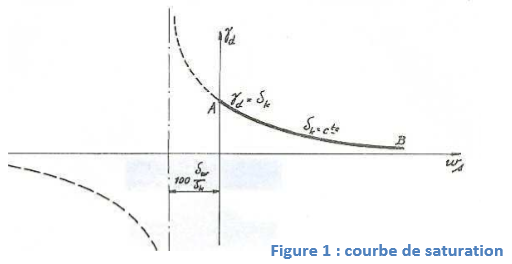
\includegraphics [scale=0.5]{pictures/cs.PNG}
\end{center}

Les points représenté entre A et B sont des états de saturation parfaite. Ceux à gauche représente des états de saturation partielle et ceux à droite, des états physique impossible.

L'art du compactage est d'identifier une teneur en eau optimale pour laquelle l'énergie donnée conduit à la compacité maximale (essai de Proctor).

\subsubsection{Essai de Proctor}

L'eau joue deux rôle dans le compactage:
\begin{itemize}
    \item Propriété lubrifiante (faible Sr): facilite la réorganisation des grains.
    \item Propriété "portance" (lorsqu'on est proche de la saturation) l'eau interstitielle reprend l'effort dynamique de compactage.
\end{itemize} 

\medskip

L'essai de Proctor: Séparer l'échantillon en plusieurs fraction (avec des w différents). Compacter chaque fraction à l'aide d'un moule cylindrique muni d'une hausse (on utilise une dame de dimension et de poids standardisés tombant d'une hauteur normalisée (une grosse dame en somme)).

On obtient pour chaque fraction: $\gamma_d$ et w. On peut trouver une relation les unissant et ainsi un optimum (On atteint pas la courbe de saturation car il reste toujours un peu d'air).

On obtient finalement un degré de compactage $D_c$:

$$ D_c = \frac{\gamma_d}{\gamma_{d,max,proctor}} $$

On remarque que la courbe obtenue dépend de l'énergie (hauteur de la dame). On distingue deux essais possible: h=30.5 cm (standard) et h=46.7 cm (modifié).

\subsection{Engin de chantier}

\begin{itemize}
    \item Rouleaux vibrants : sable et gravier
    \item Dumpers pneumatique : sols limoneux
    \item Chenillard et rouleaux à pieds de mouton : sols argileux
\end{itemize}

\section{Densification en profondeur}

\subsection{Lente pour les sols fins}

\subsubsection{Préchargement seul}

basé sur le principe de consolidation, on va charger le sol par anticipation et attendre qu'il se consolide. l'eau qu'il contient va s'extraire selon un rythme dépendant du coefficient de consolidation :

$$  c_v = \frac{k}{m_c \gamma_w} $$

\underline{Rappel:} 

\begin{center}
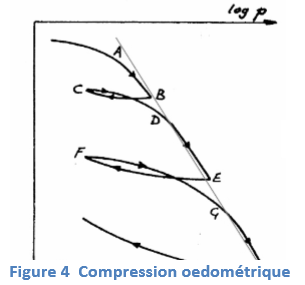
\includegraphics [scale=0.5]{pictures/oe.PNG}
\end{center}

\begin{itemize}
    \item droite des compressions vierges
    \item sol préconsolidé ou surconsolidé
    \item pression de préconsolidation $\sigma'_c$
    \item degré de surconsolidation $\sigma'_c / \sigma'_0$ (=OCR)
\end{itemize} 

\medskip

L'eau interstitielle mise sous pression va commencer à s'échapper permettant au sol de se tasser. La précharge est enlevée, le sol se décomprime légèrement (<10\% tassement).

\begin{center}
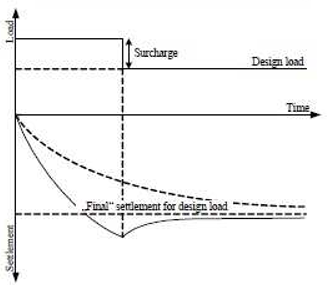
\includegraphics [scale=0.5]{pictures/a.PNG}
\end{center}

\underline{influence du temps:} 

c'est le facteur déterminant de cette méthode. Terzaghi a proposé une théorie mathématique qui donne la relation temps - niveau de consolidation.

hypothèses:
\begin{itemize}
    \item conservation de la masse
    \item principe de continuité
    \item loi de Darcy
\end{itemize} 

\medskip

$$ \frac{k}{\gamma_w}<\frac{\delta^2 u}{\delta z^2} = m_v \frac{\delta u}{\delta t} $$

on introduit le coefficient de consolidation $c_v$ (considéré comme constant) et obtient une équation différentielle de u qui dépend de z et de t.

Le tassement $s_t$ subit par une couche compressible s'exprime généralement via le degré de consolidation U défini par : $U=\frac{s_t}{s_\infty}$.

A défaut d'une solution compliquée, on obtient des expression approchées: 

\begin{itemize}
    \item $U<0.5$ : $T_v = \frac{4}{\pi} U^2$
    \item $U>0.5$ : $T_v = -0.405 ln(1-U) - 0.085$
\end{itemize} 

\medskip

On en retient de $T_v$ que la vitesse de tassement dépend de la perméabilité, de la compressibilité et du niveau de variation des contraintes mais surtout, du carré de l'épaisseur de la couche compressible. On a donc intérêt à raccourcir le chemin de percolation de l'eau.

\subsubsection{Accélération de la consolidation par drains verticaux}

L'eau circule horizontalement dans le sol mis sous pression car les drains ont un potentiel hydraulique inférieur. Avantageux car la perméabilité horizontale est souvent supérieur à la perméabilité verticale. On a donc une réduction du chemin de drainage et donc de la consolidation. 

\underline{Généralités:} 

Deux types principaux de drains: préfabriqué et "drains de sable".

La réalisation des drains provoque un remaniement de la couche de terrain et par conséquent une diminution de la perméabilité horizontale au pourtour du drain (effet "smear" = enduisage).

La résistance hydraulique du drain freine le drainage dans la mesure où sa perte de charge ne permet plus de respecter les conditions limites $u_{rw} = 0$.

Les calculs qui vont suivre prennent pour hypothèse que les drains sont cyclique. Ces formules peuvent être étendue au drains non cyclique en calculant un diamètre équivalent (ex: un prise de largeur b et épaisseur t vaut un cylindre de rayon $d_w = 2(b+t).\pi^{-1}$. 

\begin{center}
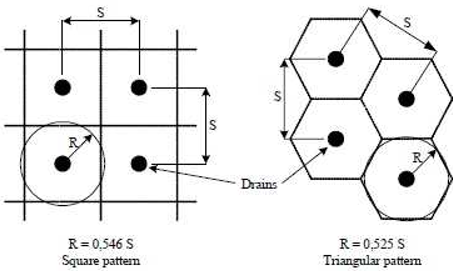
\includegraphics [scale=0.5]{pictures/plan.PNG}
\end{center}

\underline{Théorie des drains verticaux:}

hypothèse:
\begin{itemize}
    \item le mouvement radial est prépondérant
    \item cellule axisymétrique $u=u(r,z,r)$
    \item le sol est saturé (charge verticale portée par la pression interstitielle))
    \item soit charge uniformément distribuée, soit déformation provoquée par la surcharge est uniforme
    \item perméabilité du drain infinie comparée à celle du sol
    \item loi de Darcy est valide
    \item $C_h$ constant (coefficient de consolidation)
\end{itemize}

\medskip

il s'agit d'une déclinaison de la théorie de Terzaghi pour le cas 1-D vertical en un 1-D radial. On utilise l'équation de diffusion :

$$ c_h(\frac{\delta^2 u}{\delta r^2}+\frac{1}{r}\frac{\delta u}{\delta r}) = \frac{\delta u}{\delta t} $$

Conditions limites et initiales : 
\begin{itemize}
    \item $u=u_0, t=t_0$ pour tout r
    \item $u=0, r=r_w$ pour tout t
\end{itemize}

\medskip

On choisit une des deux condition mécanique à la limite supérieur du domaine: surcharge uniforme (permet la libre déformation de la surface) ou déformation uniforme (entraîne une surcharge non uniforme).

Il y a bien sur des équations simplifiées, c'est de la géotechnique ! 

Hasbo a défini $U_r$ le degré moyen de consolidation par rapport à $T_h$ un intervalle et de F(n,r,s) qui tient compte du phénomène de remaniement (s), de la résistance hydraulique (r) et de l'espacement des drains (n) : 

$$U_r = 1-exp(\frac{-sT_h}{F(n,r,s)})$$ 
$$T_h = t\frac{c_h}{d_e^2}$$ 
$$F(n,r,s) = F(n) + F(r) + F(s) = ln(\frac{n}{s})+\frac{k_h}{K_w}ln(s)-0.75+\pi z(2l-z^2)\frac{k_h}{q_w}$$ 

En mettant tout ensemble on obtient pour un drain parfait (F(s)=F(r)=0):

$$t=\frac{F(n)}{8}ln(\frac{1}{1-U_r})\frac{d^2_e}{c_h}$$

\begin{itemize}
    \item $k_h$ est la perméabilité horizontale, $k_w$ la perméabilité réduite au rayon $r_s$
    \item $q_w$ est le débit $[m^3/s]$
    \item $l$ est la longueur de drainage et $z$ est la distance du plan horizontale (0<z<2l)
    \item $U_h$ se détermine sur un graphique
\end{itemize} 

\medskip

L'évacuation par drainage verticale correspond à la théorie vue au point 3.1.1.

On peut finalement combiner les deux directions, on obtient une autre équation de diffusion:

$$c_h(\frac{\delta^2 u}{\delta r^2}+\frac{1}{r}\frac{\delta u}{\delta r}) + c_v\frac{\delta^2 u}{\delta z^2}= \frac{\delta u}{\delta t} $$ 

Un certain Carillo a démontré qu'on pouvait calculer la consolidation séparément et ensuite combiner grâce à l'équation:

$$ 1-U = (1-U_r)(1-U_v) $$ 

\underline{En pratique:}

Le coefficient majeur de consolidation implique la compression dans la direction verticale et le drainage dans la direction horizontale:

$$ c_vh = \frac{k_h(1+e_0)}{a_v\gamma_w}$$

\subsubsection{Remblai hydraulique}

Méthode utilisé en bord de mer. On pompe du sable en évitant de remonter de la vase et autre matériaux compressible. La pompe refoule le mélange d'eau et sable, les deux composants se séparent naturellement sous l'effet de la gravité.

\subsection{Rapide pour les "compactable" en profondeur}

\subsubsection{Vibro-compactage}

\underline{Généralité:} 

On transmet une énergie de vibration (effort cyclique) à un sol peu cohérent pour qu'il se compacte. Le sable sec est contractant sous l'effet du cisaillement, il aura tendance à se densifier. Le même sable saturé ne peut instantanément se réduire de volume. son comportement non drainé entraîne une augmentation de sa pression interstitielle, u augmente jusqu'à atteindre $\sigma$. La contrainte effective $\sigma'$ devient nulle et si c est nul (sol pulvérulent), la résistance au cisaillement s'annule. Il y a donc liquéfaction du sol. Il faut donc attendre que l'eau interstitielle s'évacue pour observer un tassement du sable (du à la gravité).

\underline{Granulométrie:} 

Pour réaliser cette liquéfaction,il faut suffisamment d'eau (pas un problème dans nos région) et que le matériaux respecte certains fuseaux granulométrique.

\begin{center}
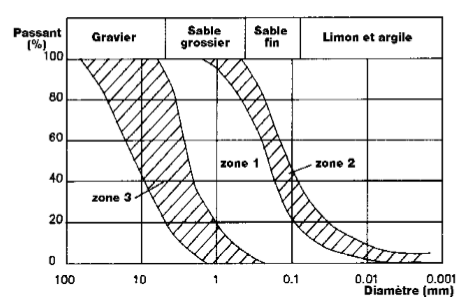
\includegraphics [scale=0.5]{pictures/gr.PNG}
\end{center}

Si le sol est trop cohérent, il n'entrera pas en liquéfaction et il sera difficile d'y enfoncer l'outil vibrant. Si la granulométrie est trop grossière, l'enchevêtrement des grains va les empêcher de se réorganiser. Il faut donc se trouver dans la zone 1.

\underline{Procédés techniques:}

\begin{itemize}
    \item Y-probe: axe verticale qui génère un effort sinusoïdal. L'énergie vibratoire réduit les forces inter-granulaires et permet d'atteindre une densité d'environ 70 à 85\%. L'angle de frottement et la rigidité du sol augmente également.
    \item Vibrolance: masselotte enfoncé à profondeur finale. Compactage réalisé en passe successive de bas en haut (volume = cylindre de 3 mètres de diamètre). L'intensité du vibreur permet de connaître en temps réel l'augmentation de la compacité du sol. On observe un cône d'affaiblissement que l'on comble au fur et a mesure. Après traitement, on règle et recompacte avec un rouleau vibrant.
\end{itemize}

\medskip

\subsubsection{Consolidation dynamique}

\underline{Généralité:}

objectif:
\begin{itemize}
    \item amélioration de la résistance au cisaillement
    \item diminution de la compressibilité
    \item amélioration de l'homogénéité du sol
    \item diminution du potentiel de liquéfaction d'un dépot de sable
\end{itemize}

\medskip 

Avantage:
\begin{itemize}
    \item moins cher
    \item mise en oeuvre d'équipements moins lourds
    \item diminution des efforts dynamique et donc des vibrations
    \item possibilité d'optimiser la procédure durant le compactage
\end{itemize} 
\medskip

Le principe est simple, laisser tomber une masse d'une certaine hauteur. L'énergie potentielle devient de l'énergie cinétique et transmet au sol une énergie de compactage (je savais pas que ça existait). On attend que les surpressions interstitielles se dissipent et on recommence. 

l'efficacité dépend de différents paramètres:
\begin{itemize}
    \item nature du sol et ses propriétés
    \item conditions de contraintes initiales
    \item hauteur piedzométrique
    \item la stratification
    \item la réponse dynamique du sous-sol
    \item la profondeur
    \item le degré de compactage exigé
    \item les vibrations induites dans les structures avoisinantes
\end{itemize}

\medskip

Les méthodes d'exécutions sont choisie en fonction de ces conditions afin d'éviter certain effets indésirable:
\begin{itemize}
    \item effet dalle: une couche dense se forme à la surface et empêche le compactage des couches inférieures.
    \item effet moustache: le sol dans le voisinage immédiat est soulevé (déplacé) plutôt que compacté.
    \item effet de refoulement latéral: le sol est déplacé latéralement le long d'une surface de rupture par cisaillement (déplacé et non compacté).
\end{itemize}

\medskip

\underline{mise en oeuvre:}

\begin{itemize}
    \item Si risque de refoulement latéral: couvrir le site d'une couche de sol granulaire pour fournir une plate forme de travail.
    \item Pilonner une première fois en lâchant un nombre prédéterminé de fois la masse en chaque noeud d'un maillage carré.
    \item Pilonner à nouveau selon un maillage différent (les coins des maillages précédent par exemple) (on parle de passe à haute énergie).
    \item Mettre à niveau la surface en utilisant des hauteurs réduite sur un maillage plus serré (repassage à faible énergie). On peut ensuite passé au moyen d'un rouleau vibrant.
    \item Exécuter un plot d'essai de compactage. Toujours vérifier durant et après exécution.
\end{itemize} 

\medskip

Formule très simple:
\begin{center}
\begin{tabular}{c|c}
    $D=\alpha \sqrt{M.h}$    & D: profondeur à atteindre \\
                             & $\alpha$:coefficient empirique $\in [0.5;0.9]$ \\
                             & M: masse \\
                             & h: hauteur de la chute
\end{tabular}
\end{center}

\medskip

\underline{Vibrations:}

On utilise un géophone tridimensionnel afin de s'assurer que les vibrations du au impactes n'endommage pas les constructions proches.

\medskip

\underline{Déplacement du sol:}

La profondeur est mesurée entre chaque coup, le sol se tasse de moins en moins, on peut ainsi observer la densification du sol et donc augmenter l'énergie spécifique pour certains point ou l'enfoncement est moindre. Il est également possible de déduire le volume total de sol déplacé, que l'on peut mettre en relation avec une moyenne brute de compression du sol (corrigée en fonction de l'effet moustache et de refoulement) afin d'obtenir la compression moyenne nette du sol.

\medskip

\underline{Contrôle de l'amélioration:} 

Il existe plusieurs essais possible:
\begin{itemize}
    \item tube piézométrique : u (pression interstitielle)
    \item Essais CPT (quelques heures après)
    \item CTP, SPT, PMT pour évaluer le compactage final (après la première passe)
\end{itemize}

\medskip

\underline{Essais dynamiques:}

Utilisé quand on ne peut pas réaliser des essais statiques (galets, rochers, ... on arrive pas a mettre la sonde pressiométrique). Technique qui consiste à mesurer la décélération de la masse résultante de l'impact pour déduire la réponse dynamique du sous-sol.

Pour les tests, il est important que la surface soit parfaitement plane. De plus il est nécessaire de mesurer:
\begin{itemize}
    \item H: la hauteur de chute
    \item Sr: l'enfoncement permanent de la masse
    \item a: l'accélération (obtenu en utilisant un accéléromètre)
\end{itemize} 
 
\medskip
 
 On obtient trois graphes:
 \begin{itemize}
     \item accélération en fonction du temps.
     \item tassement (s) en fonction de la force (F). s est obtenu en intégrant deux fois l'accélération et la force en appliquant Newton. Ce diagramme indique deux étapes, contact masse-sol parfait ou imparfait.
     \item diagramme force-déplacement obtenu par combinaison du diagramme charge-tassement.
 \end{itemize}
 
 \section{Renforcement des sols}
 
 On introduit dans le sol un matériaux aux propriété mécaniques complémentaires (matériau composite). En gros le sol est nul en traction donc on met un matériau bon en traction.
 
 \subsection{Inclusions structurelles}
 
 Ancrage, cloutage,... mais le plus répandu reste l'utilisation de pieux racines. micro-pieux (10-25 cm de diamètre) consistant en des tiges d'acier enrobées de béton. On triangule (voir schéma) pour résister en compression et en traction. Mais ça reste sensible au cisaillement et à la flexion. Souvent utilisé en sous-oeuvre dans des endroits difficiles d'accès car l'équipement est très léger (environ 3 tonnes).
 
\begin{center}
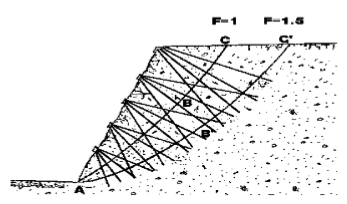
\includegraphics [scale=0.5]{pictures/b.PNG}
\end{center}

\subsection{Inclusions souples}

Utilisé dans les procédé "terre armée" et dans des applications mécaniques des géotextiles. Bref ça nous concerne pas (LAUCE1172).

\subsection{Inclusions granulaires}

\subsubsection{Colonnes ballastées}

Le but n'est pas de densifier localement le sol mais le rendre globalement plus résistant à la compression et au cisaillement (moins compressible).

\medskip

\underline{Mise en oeuvre:}

\begin{itemize}
    \item Refoulement: comme des pieux de refoulement moulés dans le sol. On enfonce un fourreau et on le retire petit à petit pendant qu'on compacte violemment pierre,gravier, sable,... par mouton à chute libre. bref on met on tape en recule et rebelotte.
    \item Lançage (substitution): on développe un trou on vient ensuite y ajouter de la pierraille depuis la surface via une torpille vibrante. (utilisable dans les remblais non évolutif).
\end{itemize}

\medskip

\underline{Les réseaux de colonnes ballastées:}

Domaine d'influence: On suppose que la cellule élémentaire est limité latéralement par une frontière fixe mais lisse et que les déformations verticales sont uniformes sur toute la hauteur.

\begin{itemize}
    \item Aire de la cellule : $A = \frac{\pi D_e^2}{4}$
    \item Aire de la colonne : $A_c = \frac{\pi D_c^2}{4}$
    \item Aire du sol : $A_s = A - A_c$
\end{itemize}

\medskip

Angle de frottement interne du ballast compacté: Durant l'avant projet, on fixe un angle de frottement interne $\phi$. 38° si le granulat est relativement fin (<50mm) et le sol d'un naturel argileux, 42° dans le cas d'un matériaux plus gros (<100 mm) et le sol d'un naturel plus limoneux.

\medskip

Rapport des modules de déformation élastique: On utilise une valeur minimale usuellement retenue (car peu d'unfo) $E'_c = 60$ MPa. Certain adoptent le module oedométrique de 100MPa (Priebe) ce qui donne en considérant le coefficient de Poisson $\nu_c = 1/3$, $E'_c=66.7$ MPa.

\medskip 

Rapport des concentrations des contraintes: La charge verticale appliquée à la surface du sol $\Delta q$ se répartit entre la colonne et le sol qui l'entoure au sein d'une cellule. On obtient la relation :

$$ \Delta q A=\Delta q_c A_c + \Delta q_s A_s $$ 

Le rapport de concentration des contraintes se définit comme : $n = \frac{\Delta q_c}{\Delta q_s}$ Caractéristique fondamental de la colonne ballastée, cette concentration se développe au fur et à mesure de l'évolution de la consolidation primaire du sol autour de l'inclusion.

\begin{center}
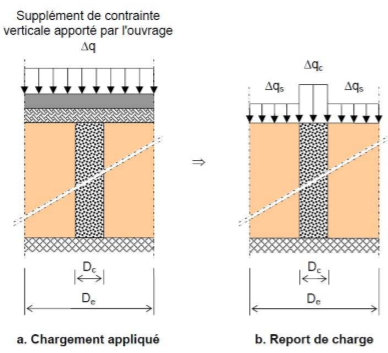
\includegraphics [scale=0.5]{pictures/27.PNG}
\end{center}

\medskip

Facteur de réduction des tassements: permet de caractériser l'efficacité du traitement.

\begin{center}
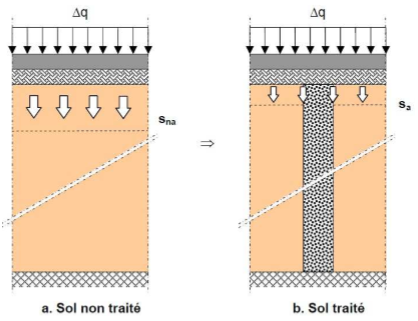
\includegraphics [scale=0.5]{pictures/28.PNG}
\end{center}

Formule très simple:
\begin{center}
\begin{tabular}{c|c}
    $\beta = \frac{S_{na}}{S_a}$    & $S_{na}$:tassement sol non traité \\
                                    & $S_a$:tassement sol traité 
\end{tabular}
\end{center}

\medskip

Relation entre n et $\beta$: On peut définir des relations particulières entre le rapport de concentration de contraintes et le facteur de réduction des tassement dans le cas de comportement purement élastique du sol et du ballast et de fondations rigides (tassement en tête des colonnes et tassement du sol identique).

$$ n = \frac{\Delta q_c}{\Delta q_s} = \frac{E_c}{E_s}$$ 

On peut faire le lien en ajoutant l'hypothèse de fondation rigide : 

$$ S_a = \frac{\Delta q_s}{E_s} H = \frac{\Delta q_c}{E_c} H$$ 

On peut en déduire que : 

$$ \beta : \frac{\delta q}{\Delta q_s}$$.

\medskip

\underline{Dimensionnement:}

Méthode empirique des abaques de Mattes et Poulos: Dans le cas d'un chargement vertical, les tassements immédiats ($s_i$) constituent la majeure partie du tassement final $(s_f)$. 

\begin{center}
\begin{tabular}{c|c}
    $s_i=\frac{Q}{L E_s}I_p$    & L:longueur de la colonne  \\
    $s_f = \frac{Q}{L E'_s}$    & $D_c$: Diamètre de la colonne \\
                                  & $E_c$: Module d'élasticité de la colonne \\
                                  & $E_s$: Module d'élasticité du sol (non drainé) \\
                                  & $E'_s$: Module d'élasticité du sol (drainé) \\
                                  & $I_p$: facteur d'influence dépendant de la rigidité relative $E_c/E_s$
\end{tabular}
\end{center}

\medskip

Méthode élastique de Balaam et Brooker: Ils ont développé une solution analytique exacte en élasticité linéaire à partir du modèle de la cellule élémentaire sous condition oenométrique. Ils obtiennent une équation pour $E_s$, qui dépend des coefficient de lamé, des modules oedométriques et du module apparent du sol une fois amélioré.

\medskip

Méthode élastoplastique de Priebe: Il crée un ensemble sol-colonnes de caractéristiques $E_s$ et $\nu_s$. Il est supposé vérifier les hypothèse suivante:

\begin{itemize}
    \item tassement en surface sont égaux ($s_{col}=s_{sol}$).
    \item matériaux constitutif colonne sont actif et les déformations de la colonne suivent celles du sol.
    \item colonne incompressible
    \item le terrain (compressible) a un comportement élastique linéaire ($E_s$ et $\nu_s$)
    \item déplacement radiaux sont nuls
    \item conservation des sections planes
\end{itemize} 

\medskip

\begin{center}
\begin{tabular}{c|c}
    $\Delta q = \Delta \sigma_{hc} - \Delta \sigma_{hs}$   
            & $\Delta \sigma_{hc}$: accroissement de la contrainte horizontale dû à $\Delta q_c$  \\
            & $\Delta \sigma_{hs}$:accroissement de la contrainte horizontale dû à $\Delta q_s$
\end{tabular}
\end{center}

Il définit également $\beta$ et n. La relation entre les deux facteurs d'amélioration permet d'aboutir à un graphe : 

\begin{center}
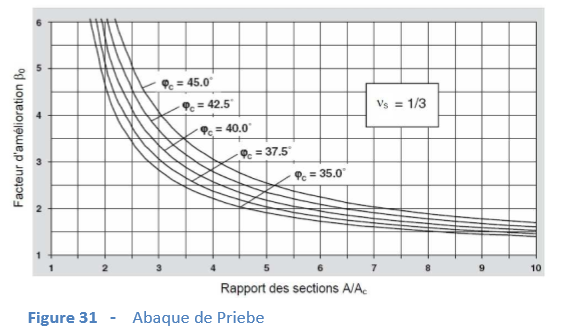
\includegraphics [scale=0.5]{pictures/pr.PNG}
\end{center}

\medskip
\underline{Mécanisme de rupture:}

\begin{center}
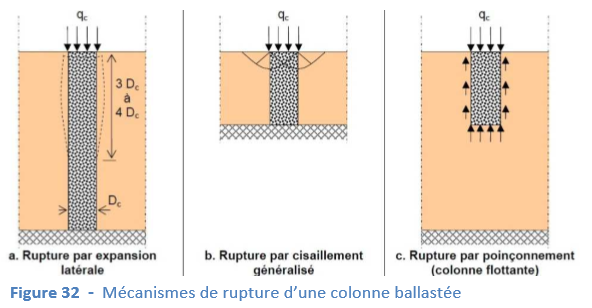
\includegraphics [scale=0.7]{pictures/32.PNG}
\end{center}

rupture par expansion latérale: le plus fréquent, contrainte axiale appliquée par le bâtiment et une contrainte latérale par le sol. Cette contrainte radiale peut être mesurée au moyen d'un pressiomètre. Le sol étant généralement purement cohésif, $p_{lim} = 5.5 c_u$. Une utilise le coefficient de butée et un coefficient de sécurité :

$$ q_c < 20 c_u + q_s$$

\medskip 

Rupture par cisaillement généralisé : colonnes courte avec rupture par cisaillement

\medskip

Rupture par poinçonnement (colonne flottante): On peut déterminer une longueur minimale ($L_min$ nécessaire pour éviter le poinçonnement. 

$$L_min = \frac{1}{4} D_c (\frac{q_c}{c_u}-9)$$
$$q_c < c_u (9+\frac{4L}{D_c}$$

\medskip

\underline{Essais de vérification:} on ne maîtrise pas parfaitement l'exécution des colonnes ni les caractéristiques du milieu hétérogène. Il convient donc de suivre ce qu'il se passe en temps réel pour adapter l'exécution. Essai de chargement à grande échelle réalisé in situ. 

L'essai à la plaque (essai statique du sol = SGT):
\begin{itemize}
    \item qualitatif: mesurer augmentation de la raideur du sol
    \item quantitatif: déterminer le module réel de réaction k
\end{itemize}

Exécuté sur un temps très cours, on est en condition non drainée pour le sol mais drainée pour les ballaste (matériaux granulaire).

\section{Stabilisation Physico-chimique}

\subsection{Stabilisants aux liants hydrauliques}

Deep soil mixing: On incorpore un coulis de ciment et on mélange, attention aux hétérogénéités.

\subsection{Congélation}

méthode à caractère temporaire.

\subsection{Jet (ou VHP) Grounting}

On utilise un jet très puissant pour déstructurer un terrain et le mélanger avec le fluide. C'est un procédé hydrodynamique terrain-coulis visant à former un "béton de sol" dans la masse de terrain.

\subsection{Les injections}

pour les sols rocheux : remplir les discontinuités (strates, fissures, ...) pour améliorer la résistance en compression, augmenter son module de déformation et réduire la perméabilité. 

Pour les sols non cohésifs : le fluide bouche les espaces poreux. (même effet).

Le type d'injection dépend de la granulométrie en présence (le fluide doit pouvoir passer entre les grains). Pour les sol rocheux, il faut faire attention de ne pas endommager le sol avec une trop grosse pression (max 80\% de la résistance au cisaillement). Pour les sols cohérent, on crée volontairement des discontinuité par une pression supérieur, cela s'appelle la fracturation hydraulique.

\subsubsection{Le tube a manchette}

On fore, on descend le tube avec un bouchon à sa base (surmonté du tube lisse). On coule la manchette par du ciment dans le pour le sceller. On ajoute dans la manchette un double obturateur pour assurer l'étanchéité. Ensuite il y a la phase du claquage ou l'on perfore le ciment pour atteindre le sol avec l'injection. Il faudra faire attention à respecter les quantités à injecter et la pression maximale. Une fois fini on enlève tout et on rince le tube pour pouvoir le réutiliser.

\medskip

les injections sont utiles dans plusieurs autres situations:
\begin{itemize}
    \item réparation de fondations ancienne
    \item relevage des structures
    \item protection d'ouvrage (on doit mettre un tunnel ou autre)
\end{itemize}

